%%%%%%%%%%%%%%%%%%%%%%%%%%%%%%%%%%%%%%%%%%%%%%%%%%%%%%%%%%%%
%%  This Beamer template was created by Cameron Bracken.
%%  Anyone can freely use or modify it for any purpose
%%  without attribution.
%%
%%  Last Modified: January 9, 2009
%%

\documentclass[xcolor=x11names,compress]{beamer}

%% General document %%%%%%%%%%%%%%%%%%%%%%%%%%%%%%%%%%
\usepackage{graphicx}
\usepackage{tikz}
\usepackage[utf8]{inputenc}
\usepackage{amsmath}
\usepackage[english]{babel}
\usetikzlibrary{decorations.fractals}
\usepackage[export]{adjustbox}
%%%%%%%%%%%%%%%%%%%%%%%%%%%%%%%%%%%%%%%%%%%%%%%%%%%%%%


%% Beamer Layout %%%%%%%%%%%%%%%%%%%%%%%%%%%%%%%%%%
\useoutertheme[subsection=false,shadow]{miniframes}
\useinnertheme{default}
\usefonttheme{serif}
\usepackage{palatino}

\setbeamerfont{title like}{shape=\scshape}
\setbeamerfont{frametitle}{shape=\scshape}

\setbeamercolor*{lower separation line head}{bg=DeepSkyBlue4} 
\setbeamercolor*{normal text}{fg=black,bg=white} 
\setbeamercolor*{alerted text}{fg=red} 
\setbeamercolor*{example text}{fg=black} 
\setbeamercolor*{structure}{fg=black} 
 
\setbeamercolor*{palette tertiary}{fg=black,bg=black!10} 
\setbeamercolor*{palette quaternary}{fg=black,bg=black!10} 

\addtobeamertemplate{footline}{\hspace{0.5cm} \insertframenumber / \inserttotalframenumber}

\renewcommand{\(}{\begin{columns}}
\renewcommand{\)}{\end{columns}}
\newcommand{\<}[1]{\begin{column}{#1}}
\renewcommand{\>}{\end{column}}
\beamertemplatenavigationsymbolsempty
%%%%%%%%%%%%%%%%%%%%%%%%%%%%%%%%%%%%%%%%%%%%%%%%%%




\begin{document}


%%%%%%%%%%%%%%%%%%%%%%%%%%%%%%%%%%%%%%%%%%%%%%%%%%%%%%
%%%%%%%%%%%%%%%%%%%%%%%%%%%%%%%%%%%%%%%%%%%%%%%%%%%%%%
\section*{\scshape}
\begin{frame}
\title{Which concepts for automatic extractive summarization?}
\author{Marie \textsc{Lenogue}, Anthony \textsc{Pena}, Clément \textsc{Tek}\\
Supervised by Florian \textsc{Boudin} and Hugo \textsc{Mougard}\\
}


\date{
	\\
	\vspace{1cm}
	April 28, 2015
}
\titlepage
\begin{figure}[!h]
	
\includegraphics[scale=0.15]{UN.png}
    
\includegraphics[scale=0.3]{lina.png}
\end{figure}
5\end{frame}

%%%%%%%%%%%%%%%%%%%%%%%%%%%%%%%%%%%%%%%%%%%%%%%%%%%%%%
%%%%%%%%%%%%%%%%%%%%%%%%%%%%%%%%%%%%%%%%%%%%%%%%%%%%%%
\begin{frame}{Table of contents}
\tableofcontents
\end{frame}

%%%%%%%%%%%%%%%%%%%%%%%%%%%%%%%%%%%%%%%%%%%%%%%%%%%%%%
%%%%%%%%%%%%%%%%%%%%%%%%%%%%%%%%%%%%%%%%%%%%%%%%%%%%%%
\section{\scshape Introduction}
\subsection{What is automatic extractive summarization?}
\begin{frame}{What is automatic extractive summarization?}
\begin{center}
Corpus\\$\downarrow$\\ Extraction of sentences subsets \\ $\downarrow$ \\Sorting of the extracted subsets \\$\downarrow$ \\Summary

\begin{figure}[!h]
	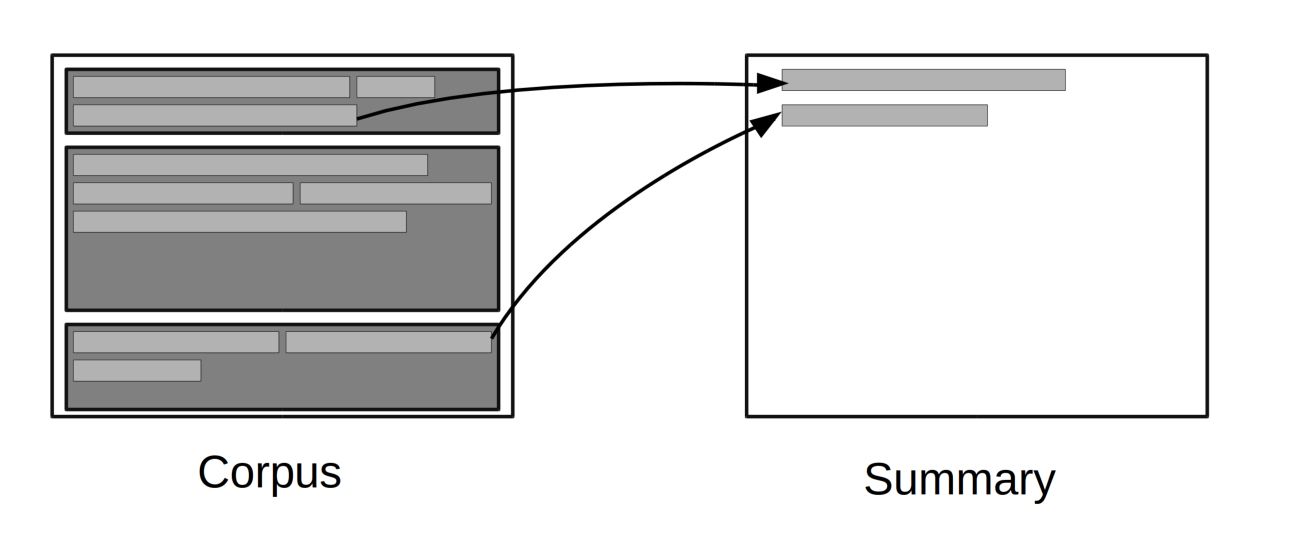
\includegraphics[scale=0.2]{first.png}
\end{figure}

\end{center}
\end{frame}
%%%%%%%%%%%%%%%%%%%%%%%%%%%%%%%%%%%%%%%%%%%%%%%%%%%%%%
%%%%%%%%%%%%%%%%%%%%%%%%%%%%%%%%%%%%%%%%%%%%%%%%%%%%%%
\subsection{What is a concept?}
\begin{frame}{What is a concept?}
A concept is an entity, often weighted according to its significance in the study.\\
\vspace{1cm}
It can be:
\begin{itemize}
\item A bigram of words
\item A nominal group
\item A dependancies tree
\item ...
\end{itemize}
\end{frame}

%%%%%%%%%%%%%%%%%%%%%%%%%%%%%%%%%%%%%%%%%%%%%%%%%%%%%%
%%%%%%%%%%%%%%%%%%%%%%%%%%%%%%%%%%%%%%%%%%%%%%%%%%%%%%
\subsection{ROUGE}
\begin{frame}{ROUGE - Recall-Oriented Understudy for Gisting Evaluation}
\begin{itemize}
\item Measure system for automatic summarization \\
\item Compares generated summaries with a set of references (summaries) produced by humans
\item Used in competitions like TAC (Text Analysis Conference) and DUC (Document Understanding Conference)
\end{itemize}
\end{frame}


%%%%%%%%%%%%%%%%%%%%%%%%%%%%%%%%%%%%%%%%%%%%%%%%%%%%%%
%%%%%%%%%%%%%%%%%%%%%%%%%%%%%%%%%%%%%%%%%%%%%%%%%%%%%%
\section{\scshape State-of-Art}
\subsection{Concepts}
\begin{frame}{Concepts}
Only bigrams of words are considered in literature:\\
\begin{itemize}
\item Fast processing and deliver good results\\
\item No work found about the importance of choosing textual units for concepts
\end{itemize}

How can we evaluate the choice of the type of concept?

\end{frame}


%%%%%%%%%%%%%%%%%%%%%%%%%%%%%%%%%%%%%%%%%%%%%%%%%%%%%%
%%%%%%%%%%%%%%%%%%%%%%%%%%%%%%%%%%%%%%%%%%%%%%%%%%%%%%

\subsection{Extraction by linear optimization}
\begin{frame}{Extraction by linear optimization}
\textsc{D. Gillick} \& \textsc{B. Favre} : \textit{A scalable global model for summarization}, June 2009.\\
\vspace{1cm}
	\begin{figure}[!h]
    	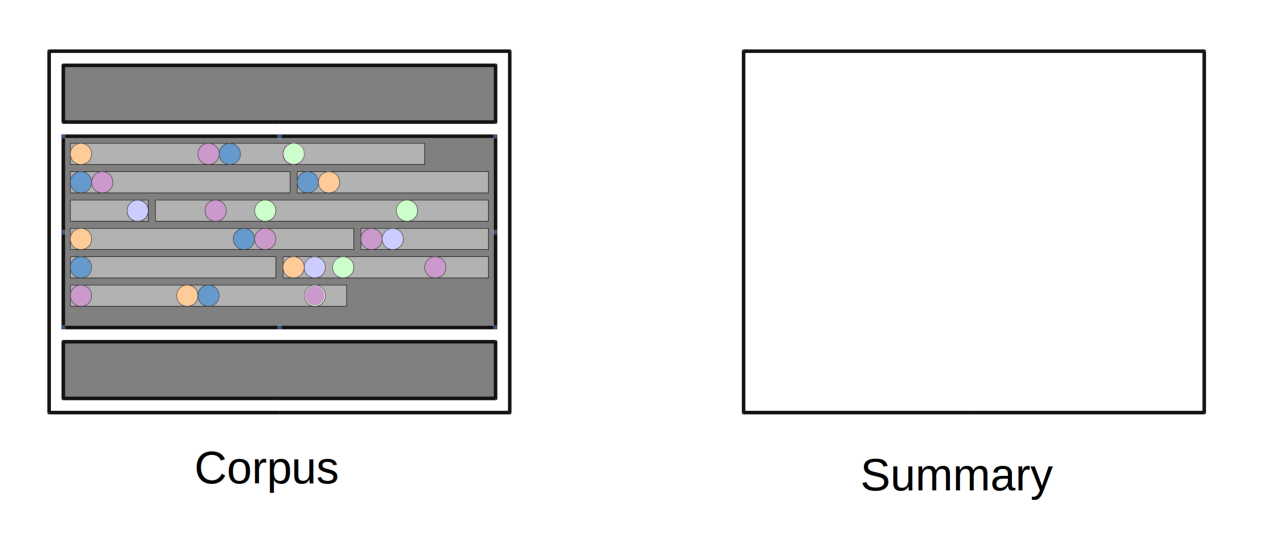
\includegraphics[scale=0.25]{1.png}
    \end{figure}
\end{frame}

%%%%%%%%%%%%%%%%%%%%%%%%%%%%%%%%%%%%%%%%%%%%%%%%%%%%%%

\begin{frame}{Extraction by linear optimization}
\textsc{D. Gillick} \& \textsc{B. Favre} : \textit{A scalable global model for summarization}, June 2009.\\
\vspace{1cm}
	\begin{figure}[!h]
    	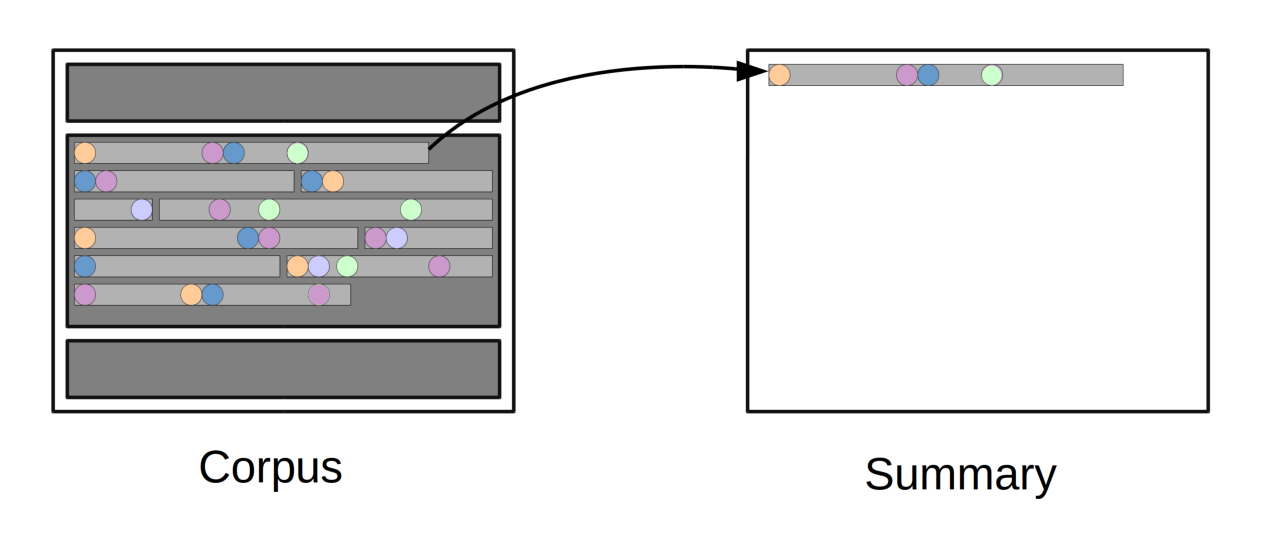
\includegraphics[scale=0.25]{2.png}
    \end{figure}
\end{frame}

%%%%%%%%%%%%%%%%%%%%%%%%%%%%%%%%%%%%%%%%%%%%%%%%%%%%%%

\begin{frame}{Extraction by linear optimization}
\textsc{D. Gillick} \& \textsc{B. Favre} : \textit{A scalable global model for summarization}, June 2009.\\
\vspace{1cm}
	\begin{figure}[!h]
    	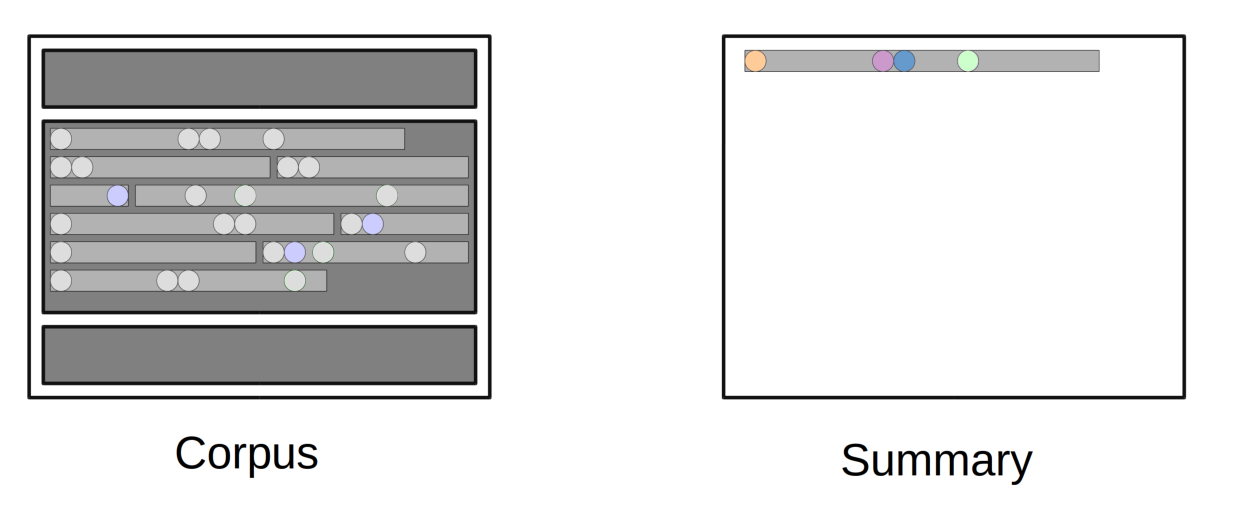
\includegraphics[scale=0.25]{3.png}
    \end{figure}
\end{frame}

%%%%%%%%%%%%%%%%%%%%%%%%%%%%%%%%%%%%%%%%%%%%%%%%%%%%%%

\begin{frame}{Extraction by linear optimization}
\textsc{D. Gillick} \& \textsc{B. Favre} : \textit{A scalable global model for summarization}, June 2009.\\
\vspace{1cm}
	\begin{figure}[!h]
    	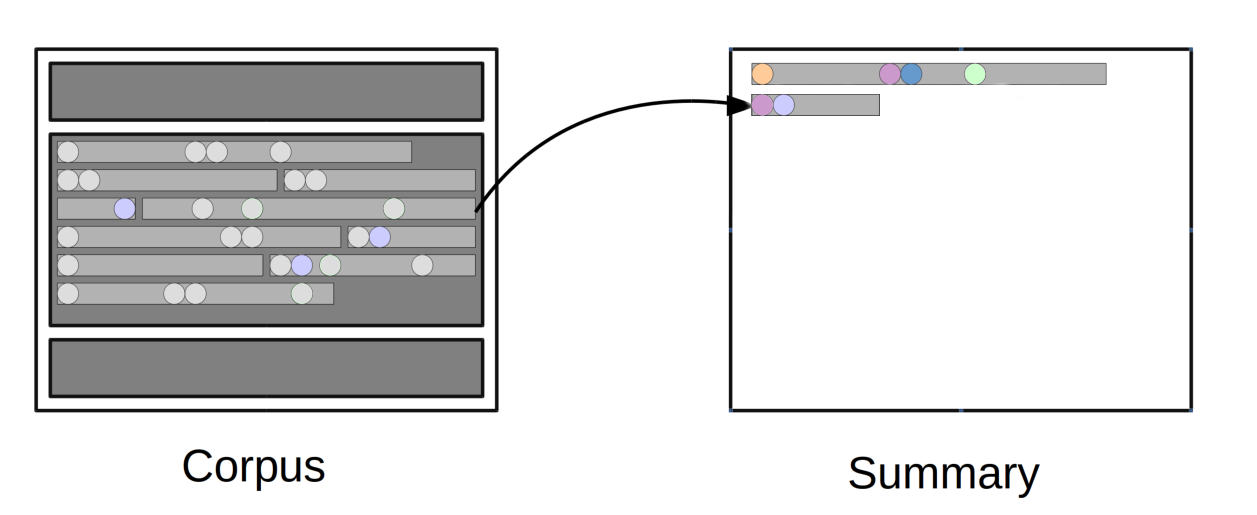
\includegraphics[scale=0.25]{4.png}
    \end{figure}
\end{frame}

%%%%%%%%%%%%%%%%%%%%%%%%%%%%%%%%%%%%%%%%%%%%%%%%%%%%%

\begin{frame}{Extraction by linear optimization}
\textsc{D. Gillick} \& \textsc{B. Favre} : \textit{A scalable global model for summarization}, June 2009.\\
\vspace{1cm}
Maximize the objective function:\\
\[\sum_{i} w_i c_i\]\\
$c$ : presence of the concept (binary)\\
$w$ : weight of the concept
\end{frame}

%%%%%%%%%%%%%%%%%%%%%%%%%%%%%%%%%%%%%%%%%%%%%%%%%%%%%%
%%%%%%%%%%%%%%%%%%%%%%%%%%%%%%%%%%%%%%%%%%%%%%%%%%%%%%
\subsection{Regression model}
\begin{frame}{Regression model}
\textsc{C. Li , X. Qian} \& \textsc{Y. Liu} : \textit{Using Supervised Bigram-based ILP for Extractive Summarization}, August 2013.\\
\vspace{1cm}
Use several indicative features at word or sentence level:
\begin{itemize}
\item Bigram frequency in the given subject
\item Stopwords ratio in the bigram
\item Similarity with the subject title
\item Similarity of the sentence with the concatenation of the subject title and description
\item Sentence position in the text
\item Is it a paragraph beginning? (binary)\\
\end{itemize}
\end{frame}

%%%%%%%%%%%%%%%%%%%%%%%%%%%%%%%%%%%%%%%%%%%%%%%%%%%%%%
%%%%%%%%%%%%%%%%%%%%%%%%%%%%%%%%%%%%%%%%%%%%%%%%%%%%%%
\section{\scshape Tries and results}
\subsection{Grouping}
\begin{frame}{Grouping}
Nominal locutions :
\begin{itemize}
\item Point of view
\item On my way
\item "Suprême de volaille"
\item ...
\end{itemize}
Detected as trigram, but represent only one entity. What can we do?
\begin{itemize}
\item Group in a single word
\item Add a locution dictionary
\end{itemize}
\end{frame}

%%%%%%%%%%%%%%%%%%%%%%%%%%%%%%%%%%%%%%%%%%%%%%%%%%%%%%
%%%%%%%%%%%%%%%%%%%%%%%%%%%%%%%%%%%%%%%%%%%%%%%%%%%%%%
\begin{frame}{Grouping}
Grammatical group :
\begin{itemize}
\item subject
\item verb
\item subject + verb
\item ...
\end{itemize}
Try to detected some logical group.
\begin{itemize}
\item Not accurate
\item Not effective
\item Few similarity between documents
\end{itemize}
\end{frame}

%%%%%%%%%%%%%%%%%%%%%%%%%%%%%%%%%%%%%%%%%%%%%%%%%%%%%%
%%%%%%%%%%%%%%%%%%%%%%%%%%%%%%%%%%%%%%%%%%%%%%%%%%%%%%
\subsection{Weighting}
\begin{frame}{Weighting}
Another lead would be changing the weighting of the concepts.
Currently :
\begin{itemize}
\item Frequency of occurrence
\item Extraction of the sentences with the largest weight
\end{itemize}
Is it the best we can do?
\begin{itemize}
\item Problem: Dependence on the corpus
\item In our case: corpus of journalistic articles. Add weight on the beginning and the end?
\item More weight on quotes?
\end{itemize}
\end{frame}

%%%%%%%%%%%%%%%%%%%%%%%%%%%%%%%%%%%%%%%%%%%%%%%%%%%%%%
%%%%%%%%%%%%%%%%%%%%%%%%%%%%%%%%%%%%%%%%%%%%%%%%%%%%%%
\subsection{Problems}
\begin{frame}{Problems}
\begin{itemize}
\item Amount of data
\item Time to generate summary
\item Time to generate scores
\item Impossible to generate best one by generating all possibilities (between 551,300 and 319,195,444,750)
\end{itemize}
\end{frame}

%%%%%%%%%%%%%%%%%%%%%%%%%%%%%%%%%%%%%%%%%%%%%%%%%%%%%%
%%%%%%%%%%%%%%%%%%%%%%%%%%%%%%%%%%%%%%%%%%%%%%%%%%%%%%
\begin{frame}{Comparison between State of art and gold}
	\begin{figure}[!h]
    	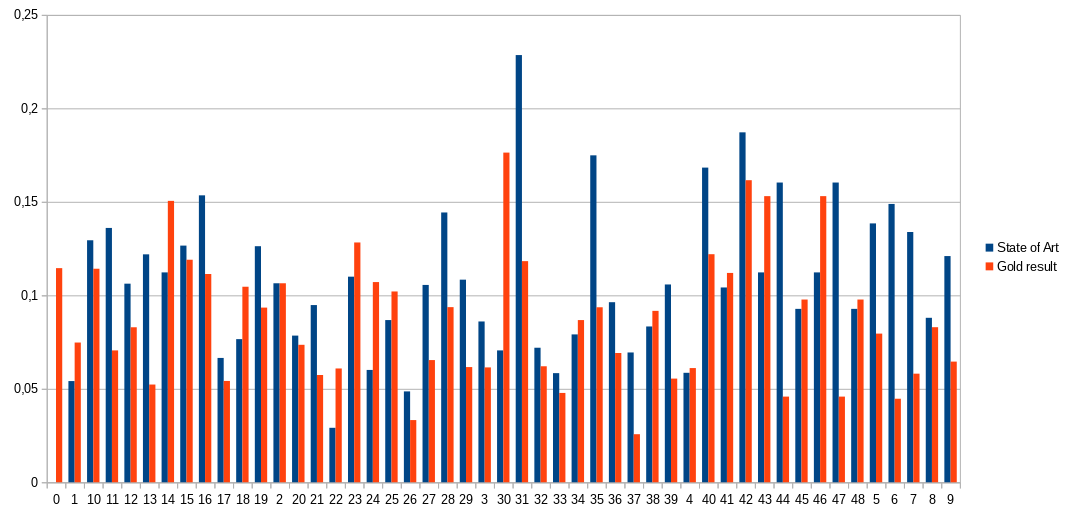
\includegraphics[width=1\linewidth]{graph.png}
    \end{figure}
\end{frame}

%%%%%%%%%%%%%%%%%%%%%%%%%%%%%%%%%%%%%%%%%%%%%%%%%%%%%%
%%%%%%%%%%%%%%%%%%%%%%%%%%%%%%%%%%%%%%%%%%%%%%%%%%%%%%
\section{\scshape Conclusion}
\begin{frame}{Conclusion}

\begin{itemize}
\item 2 ALMA and 1 ATAL for an optimization problem
\item Not supervised method
\item Is it better to improve the ROUGE score? Or satisfy human evaluation?
\end{itemize}
\begin{itemize}
\item Usage of an optimization solver
\item Make concessions to optimize time over very few improvement in quality
\end{itemize}
\end{frame}
\end{document}